\documentclass[output=paper]{LSP/langsci} 
\ChapterDOI{10.5281/zenodo.1291936}
\author{Mirela-Ştefania Duma\lastand Cristina Vertan\affiliation{University of Hamburg, Germany} }
\title{Integration of machine translation in on-line multilingual applications: Domain adaptation} 
\abstract{Large amounts of bilingual corpora are used in the training process of statistical machine translation systems. Usually a general domain is used as the training corpus. When the system is tested using data from the same domain, the obtained results are satisfactory, but if the test set belongs to a different domain, the translation quality decreases. This is due to insufficient lexical coverage, wrong choice in case of polysemous words, and differences in discourse style between the two domains. Thus, the need to adapt the system is an ongoing research task in machine translation. Some challenges in performing domain adaptation are to decide which part of the system requires adaptation and to choose what method needs to be applied. In this paper, we used language model interpolation as a domain adaptation method and proved that it is a fast state of the art method that can be used in building adapted translation systems even when sparse domain specific material is available (i.e. especially in the case of low-resourced language pairs). The best improvement was of 15 \textsc{bleu} points over the baseline system.}
\maketitle

\shorttitlerunninghead{Integration of machine translation in on-line multilingual applications}
\begin{document}

%mduma@informatik.uni-hamburg.de  
%cristina.vertan@uni-hamburg.de 


\section{Introduction}\label{sec:dumavertan:1}

As a response to the increased need of managing data available on-line, traditional content management systems extended their functionality by offering a web front-end facility, and more recently by including cloud services. In this article we will refer to this type of system as Web Content Management System (\textsc{wcms}). 

Existent \textsc{wcms}s focus on storage of documents in databases and provide mostly full-text search functionality. These types of systems have limited applicability, due to two reasons: 

\begin{itemize}
\item 
data available online is often multilingual and 
\item 
documents within a \textsc{cms} are semantically related (share some common knowledge, or belong to similar topics). 
\end{itemize}

In short, in production environments, currently available \textsc{cms}s do not exploit modern techniques from information technology like text mining, the semantic web or machine translation. Current initiatives, such as the ``Multilingual Web-\textsc{lt}'' (\url{http://www.multilingualweb.eu/}), are now developing standards and best practices for dealing with multilingual content on the Web, but this has not yet been systematically applied to \textsc{CMS}s.

The \textsc{ict psp eu} project \textsc{atlas} -- Applied Technology for Language-Aided \textsc{cms} (\url{http://www.atlasproject.eu}) -- aims to fill this gap by providing three innovative Web services within a \textsc{wcms}. These three Web services, i-Librarian, EUDocLib and i-Publisher, are not only thematically differentiated, but  also offer  different levels of intelligent information processing. 

The \textsc{atlas} \textsc{wcms} makes use of state-of-the-art text-technological methods in order to extract information and cluster documents according to a given hierarchy. A text summarization module and a machine translation engine as well as a cross-lingual semantic search engine are embedded.  

Currently the system is able to handle six languages (Bulgarian, English, German, Greek, Polish and Romanian) from four language families. However, the chosen framework allows other languages to be added at a later point. 

  The focus of this paper is on the machine translation engine within the \textsc{atlas} project and on performing domain adaptation which gives significant improvements over the baseline system when evaluated. It should also be stated that the aim of the \textsc{atlas} project is to adapt state-of-the-art methods in language technology with the purpose of being integrated into a content management system, thus the project is not only a research project, but also a product-oriented one. Our attention focused on selecting the most adequate state-of-the-art method in domain adaptation for machine translation.

In natural language processing, the notion of ``domain'' could refer to the genre, the text type or the style of a document \citep{Lee2001}. In this paper, we use the definition from \citet[Chapter~3]{Plank2011} where a domain is defined by a corpus. The problem of domain adaptation could be formulated as follows: given a large amount of bilingual source data (training data) and a small amount of target data, the purpose of the domain adaptation task is to build a system that has a good performance when evaluated on test sets that belong to the target domain. We use the terms source domain and out-of-domain interchangeably. Also, the terms target domain and in-domain are used interchangeably.

  The remainder of this paper is organized as follows. In \secref{sec:dumavertan:2}, the \textsc{atlas} Content Management System is described with details on the integration of machine translation into the \textsc{atlas} system. \secref{sec:dumavertan:3} presents the state of the art in domain adaptation for statistical machine translation (\textsc{smt}) with insight on the limitations of the current methods. The next section introduces the baseline translation system we used and the resources needed in order to build it. The experiments we performed in domain adaptation are presented in \secref{sec:dumavertan:5}. We conducted two types of experiments: firstly, we identified a state of the art domain adaptation method that is easy to use and gives significant improvements over the baseline. Then, after deciding on the method, we performed various experiments on different domains from the \textsc{atlas} project and on different language pairs. The results are also presented in this section. The conclusions are presented in the last section.

\section{The ATLAS content management system}\label{sec:dumavertan:2}

The core online service of the \textsc{atlas} platform is i-Publisher, a powerful web-based instrument for creating, running and managing content-driven Web sites. It integrates language-based technologies to improve content navigation, e.g. interlinking documents based on extracted phrases, words and names, providing short summaries and suggesting categorization concepts. Currently two different thematic content-driven websites, i-Librarian and EUDocLib, are being built on top of the \textsc{atlas} platform, using i-Publisher as the content management layer. i-Librarian is intended to be a user-oriented website which allows visitors to maintain a personal workspace for storing, sharing and publishing various types of documents and to have them automatically categorized into appropriate subject categories, summarized and annotated with important words, phrases and names. EUDocLib is planned as a publicly accessible repository of \textsc{eu} legal documents from the \textsc{eur-lex} collection with enhanced navigation and multilingual access. 

The i-Publisher service:

\begin{itemize}
\item 
is mainly targeted at small enterprises and non-profit organizations, 
\item 
gives the ability to use a point-and-click interface to build content-driven websites which provide a wide set of pre-defined functionalities and whose textual content is automatically processed, i.e.\ categorized, summarized, annotated, etc., 
\item 
enables publishers, information designers and graphic designers to easily collaborate, 
\item 
aims at saving authors, editors and other contributors valuable time by automatically processing textual data and allowing them to work together to produce high quality content. The last evaluation round of the service indicates that users indeed see the benefit of \textsc{lt}-Technologies embedded into the system.
\end{itemize}

The i-Librarian service:

\begin{itemize}
\item 
addresses the needs of authors, students, young researchers and readers, 
\item 
gives the ability to easily create, organize and publish various types of documents, 
\item 
allows users to find similar documents in different languages, to share their own work with other people, and to locate the most relevant texts from large collections of unfamiliar documents.
\end{itemize}

The EUDocLib service is a particular refinement of i-Librarian targeted at the management of documents from the European Commission.

The services described above are supported through intelligent language technology components like automatic classification, named entity recognition and information extraction, automatic text summarization, machine translation and cross-lingual information retrieval. These components are integrated into the system in a brick-like architecture, which means that each component is building on top of the preceding one. The baseline brick is the language processing pipeline component which ensures homogeneous 
linguistic processing of all documents independent of their language \citep{BelogayEtAl2011}. A processing pipeline for a given language includes a number of existing tools, adjusted and/or fine-tuned to ensure their interoperability. In most respects, a language processing pipeline does not require development of new software modules, but rather a combination of existing tools. The core \textsc{atlas} software package is distributed under the \textsc{gpl} license. \textsc{lt}-plug-ins like the language processing chains or the \textsc{mt}-engine follow a commercial licensing. iLibrarian is available as a web service and it has unrestricted access.

\subsection{Machine translation in the ATLAS system}\label{sec:dumavertan:2.1}

Machine Translation is a key component of the \textsc{atlas} system. The development of the engine is particularly challenging as the translation should be applicable to different domains. Additionally, the considered language pairs belong to the low resourced group,\footnote{See \href{https://webmail.rrz.uni-hamburg.de/services/go.php?url=http://www.meta-net.eu/whitepapers & _t=1367956882 & _h=qm2othGZINLgZG6IS2rxpecefDQ}{http://www.meta-net.eu/whitepapers}.} for which bilingual training and test material is available in limited amount.

The machine translation engine is integrated in two distinct ways into the \textsc{atlas} platform:

\begin{itemize}
\item 
for the i-Publisher Service (a generic platform for generating websites), the \textsc{mt} serves as a translation aid tool for publishing multilingual content. Text is submitted to the translation engine and the result is subject to human post-processing
\item 
for i-Librarian and EUDocLib (dedicated Web services for collecting documents), the \textsc{mt}-engine provides a translation for evaluation, which means that the user retrieving documents in different languages will use the engine in order to get a clue about the documents, and decide if he will store them. If the translation is considered acceptable it will be stored in the database
\end{itemize}

The integration of a machine translation engine into a web-based content management system in general, and into the \textsc{atlas} system in particular, presents several challenges from the user's point of view, among which we mention two challenges that were dealt with within the \textsc{atlas} system:

\begin{enumerate}
\item   
The user may retrieve documents from different domains. Domain adaptation is a major issue in machine translation, and in particular in corpus-based methods. Poor lexical coverage and false disambiguation are the main issues when translating documents out of the training domain;
\item
The user may retrieve documents from various time periods. As language changes over time, language technology tools developed for modern languages do not work equally well on diachronic documents. 
\end{enumerate}

With the currently available technology, it is not possible to provide a translation system which is domain and language variation independent and works for multiple heterogeneous language pairs. Therefore, our approach envisages a system of user guidance, so that the availability and the foreseen system performance are transparent at any time.

For the \textsc{mt}-engine of the \textsc{atlas} system we decided on a hybrid architecture combining Example-Based Machine Translation (\textsc{ebmt}) \citep{Gavrila2011} and statistical machine translation (\textsc{smt}) \citep{KoehnEtAl2007} at the phrase-based level (no syntactic trees will be used). An original approach of our system is the interaction of the \textsc{mt}-engine with other modules of the system:

\begin{itemize}
\item 
The document categorization module assigns to each document one or more domains. For each domain the system administrator has the possibility to store information regarding the availability of a corresponding specific training corpus. If no specific trained model for the respective domain exists, the user is provided with a warning that the translation may be inadequate with respect to the lexical coverage.
\item 
The output of the summarization module is processed in such a way that ellipses and anaphoras are omitted, and lexical material is adapted to the training corpus.
\end{itemize}

\begin{figure}[h]
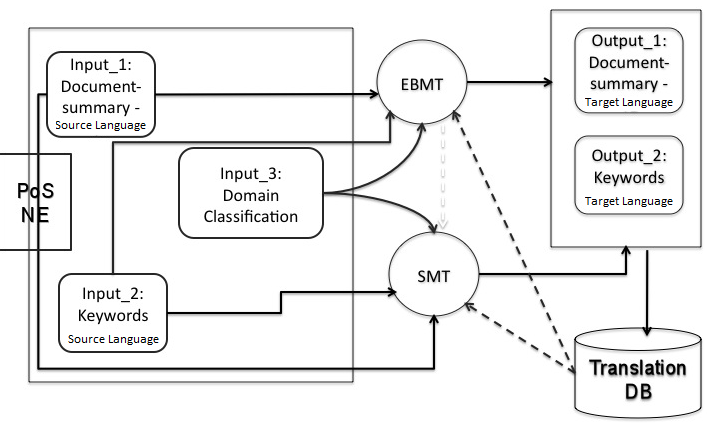
\includegraphics[width=0.6\textwidth]{figures/DumaVertanF1.png}
\caption{System architecture for the \textsc{atlas}-engine}
\label{fig:dumavertan:1}
\end{figure}

The information extraction module provides information about document me\-tadata including publication age. For documents previous to 1900 we will not provide a translation, explaining to the user that in absence of a training corpus the translation may be misleading.

The domain and dating restrictions can be changed at any time by the system administrator when an adequate training model is provided. The described architecture is presented in \figref{fig:dumavertan:1}.

  In order to perform domain adaptation we collected domain specific corpora for 13 upper domains in the categorization tree embedded in the \textsc{atlas} system and performed various experiments to choose a fast and easy to use domain adaptation method that can significantly improve the translation. 

\section{State of the art in domain adaptation for Statistical Machine Translation}\label{sec:dumavertan:3}

Domain adaptation (\textsc{da}) can be classified by taking into consideration the models that are adapted, the resources that are used or the type of supervision used.

  In the following table, multiple types of approaches are presented. The numbers of the papers that appear after the table are given in the column ``Reference'' according to the approach the paper uses in adaptation.

\begin{table}
\begin{tabular}{lll}
\lsptoprule
Approach &  Type &  Reference \\
\midrule
{Model} &  Word alignment model  & 2\\
						& Language model& 1, 3, 4, 6, 8 \\
						& Translation model & 3, 4, 5, 7, 8 \\
						& Reordering model  & 4, 7, 9 \\
\\
{Resources} &  Monolingual corpora &   5, 6, 7\\
						& Parallel corpora & 1, 2, 3, 4, 6, 9\\
						& Comparable corpora & 5 \\
						& Web-crawled data & 8 \\
\\
{Supervision} & Supervised &  1, 2, 3, 4, 8, 9\\
						& Unsupervised& 5, 7 \\
						& Semi-supervised  & 6 \\
\lspbottomrule
\end{tabular}
\caption{Classification of Domain Adaptation approaches for \textsc{smt}}
\label{tab:dumavertan:1}
\end{table}

In the following, the state of the art in domain adaptation for statistical machine translation (\textsc{smt}) is presented with papers sorted chronologically by year of publication. All papers evaluated their methods using one or more evaluation metrics and the most common metric used was \textsc{bleu} \citep{PapineniEtAl2002}.

\begin{enumerate}
\sloppy
\item 
An \textsc{unsupervised language model adaptation} method is explored in \citet{ZhaoEtAl2004} where structured query models are used. Translations are obtained using a baseline translation system that uses a general language model. Then the hypotheses from the output are converted into queries with the aim of retrieving similar sentences from very large news documents collections. Using these retrieved sentences, a language model (\textsc{LM}) is built and linearly interpolated with the baseline language model. The final step consists in using the interpolated language model to produce new translations. 
\item 
Experiments in \textsc{alignment adaptation} were described in \citet{WuEtAl2005} where out-of-domain data is used in order to get better results when performing in-domain word alignment. In their work, an alignment model is trained using the out-of-domain corpus and another alignment model is trained using the in-domain corpus (size of out-of-domain {\textgreater}{\textgreater} size of in-domain). A new alignment model results by interpolating the two models. 
\item 
Multiple experiments in domain adaptation for \textsc{smt} were explored by \citet{Koehn2007}. The baseline systems were trained using different methods: using only out-of-domain data, using only in-domain data and using concatenated out-of-domain and in-domain data. Among these three baselines the best \textsc{bleu} score was obtained using the concatenated data. The adaptation methods used were: only use the in-domain data to build the language model, interpolate the \textsc{lm} estimated from out-of-domain data with the \textsc{lm} estimated from in-domain data, use both language models as separate features with weights set using \textsc{mert}, and the last method made use of \textsc{factored translation models} where two decoding paths corresponding to each translation table are used. 
\item 
In \citet{ChenEtAl2008} n-best hypotheses are used for \textsc{language, translation and reordering model adaptation}. Each hypothesis holds phrase alignment information that is useful in the word reordering for the source text. The best word reordering for a source text is the one with the highest posterior probability. The source sentences are reordered taking into consideration the best word reordering. The weights of the decoder are optimized using the reordered source sentences. 
\item 
One approach to \textsc{translation model adaption} relies on using \textsc{comparable corpora}.\footnote{Texts that have the same topic and similar content.} In \citet{SnoverEtAl2008}, monolingual target data is used in the improvement of an \textsc{smt} system. The method consists in using multiple texts in the target language that have a similar topic as the source language document that will be translated. The documents are used to increase the probability of generating texts that are similar to the comparable document. 
\item 
The use of a \textsc{domain dictionary} and \textsc{monolingual corpora} is explored in \citet{WuEtAl2008}. The out-of-domain data is used in estimating a language model and constructing a phrase table, probabilities are assigned to entries in the in-domain translation dictionary, an in-domain phrase table is constructed, and the two phrase tables are combined. If in-domain target data is available, a language model is estimated and \textit{combined} with the out-of-domain one. If in-domain source data is available, the already built model is used in translating the data, thus obtaining a synthetic corpus that is added to the training data. 
\item 
\textsc{Monolingual resources} are also explored in \citet{Bertoldi2009}. The approaches pursued are: use the baseline translation system to generate synthetic bilingual data, use the generated data for translation and reordering model adaptation, and use the synthetic texts or given target texts for language model adaptation. 
\item 
Recent work in \textsc{DA} for\textsc{sma} focuses on using web-crawled data for building language models, improving translation models, tuning and testing. In \citet{PecinaEtAl2011} and \citet{PecinaEtAl2012}, domain-specific data is obtained by web-crawling. The basic workflow of their work is: use focused web-crawling, text normalization, language identification, document clean-up and near-duplicate detection. 
\item 
\citet{LingEtAl2011} use \textsc{weighted alignment matrices for reordering modeling.} These matrices encode all possible alignments and generate better phrase-tables. The alignment matrix is used to create the translation model and the 1-best alignment to generate the reordering model. In their paper, two algorithms to generate the reordering model are presented: one uses the alignments for the phrase pairs, and the other algorithm makes use of the contextual information of the phrase pairs.
\end{enumerate}

In \figref{fig:dumavertan:2}, a domain adaptation setup for statistical machine translation is presented.

\begin{figure}
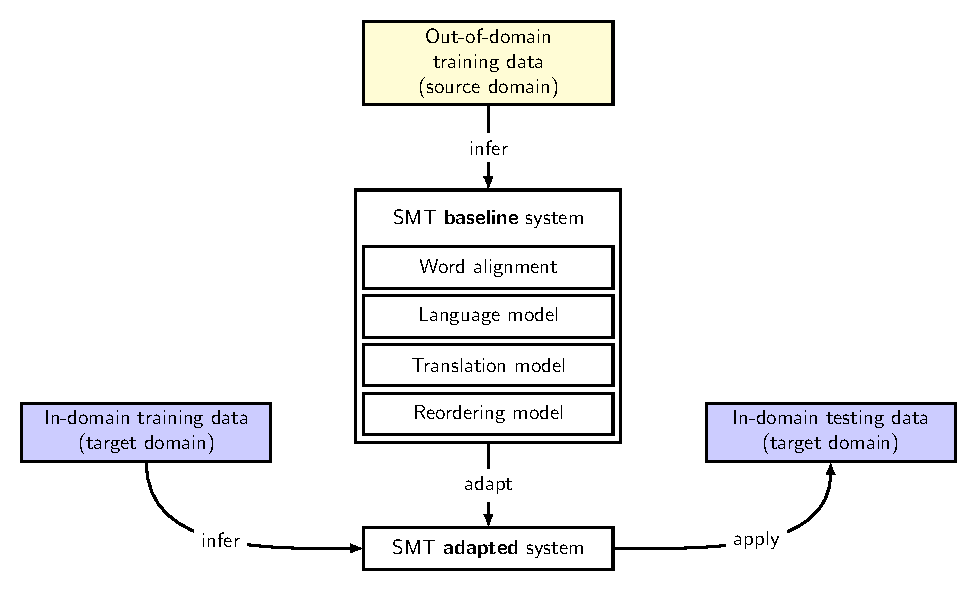
\includegraphics[width=\textwidth]{figures/DumaVertanF2.pdf}
\caption{Domain adaptation setup. Figure adapted from \citet[Chapter~3]{Plank2011} where a \textsc{da} setup is presented in the task of parser adaptation. The adapted system is made up of the same type of models as the baseline system, but these models were omitted in the drawing due to the fact that one or more models can be adapted.}
\label{fig:dumavertan:2}
\end{figure}

\section{The baseline translation system}\label{sec:dumavertan:4}
The experiments were run using the widely-used open-source toolkit Moses.\footnote{\url{http://www.statmt.org/moses/index.php?n=Main.HomePage}} Moses is a statistical machine translation toolkit which utilizes large parallel corpora in order to train the translation system. In our experiments, we used the phrase-based translation model provided by the Moses system. The training pipeline\footnote{\url{http://www.statmt.org/moses/?n=Moses.Baseline}} consists of the following steps: pre-processing the data by tokenizing, true casing and cleaning using tools from the Moses toolkit, followed by language model training and translation training where a word-alignment is performed, phrases are extracted and multiple scores are computed. For the language model training, we chose the \textsc{srilm} toolkit,\footnote{\url{http://www.speech.sri.com/projects/srilm/download.html}} which is also open-source. It builds statistical language models and it also offers the possibility of interpolating language models. As for the word-alignments, they were performed using \textsc{giza++},\footnote{\url{http://code.google.com/p/giza-pp/}} a commonly used tool for word alignments. Because of the fact that this tool runs slowly on long sentences or fails to align them, we chose to work with a maximum sentence length of 50 words.

In order to train a statistical machine translation system, parallel corpora were needed. The \textsc{jrc}-Acquis\footnote{\url{http://ipsc.jrc.ec.europa.eu/index.php?id=1989}} corpus is a multilingual parallel corpus for 22 European languages consisting of paragraph alignments for 231 pairs\footnote{\url{http://langtech.jrc.ec.europa.eu/Documents/070622\_Poster\_JRC-Acquis.pdf}} of languages. The data is made up of a selection of European Union documents referred to as Acquis. This term identifies the body of common rights and obligations that bind all the member states of the European Union. The choice of using this corpus is motivated by the fact that it is freely available, it is sufficiently large and it contains aligned corpora for all the language pairs within the \textsc{atlas} project. 


The experiments were evaluated using the common \textsc{bleu} evaluation metric which uses n-grams counts. 

\section{Experiments in domain adaptation}\label{sec:dumavertan:5}

In order to investigate current methods of domain adaptation, experiments were performed that were inspired by the work presented in \citet{Koehn2007}. In their work, the language pair French--English was used, with the Europarl corpus  used as out-of-domain date. The in-domain data was made up of the News Commentary corpus. The \textsc{bleu} scores for each of the adaptation methods proposed are presented in \tabref{tab:dumavertan:2}. 

\begin{table}
\begin{tabular}{lr}
\lsptoprule
 {Method} & {\textsc{bleu}}\\
 \midrule
 Large out-of-domain training data & 25.11\\
 Small in-domain training data & 25.88\\
 Combined training data & 26.69\\
 Language model interpolation & 27.12\\
  Two language models & 27.30\\
 In-domain language model & 27.46\\
 Two translation models & 27.64\\
\lspbottomrule
\end{tabular}
\caption{\textsc{bleu} scores for the experiments from \citet{Koehn2007}}
\label{tab:dumavertan:2}
\end{table}

From the seven experiments conducted by \citet{Koehn2007}, we selected three experiments that can be easily reproduced (combined training data, in-domain language model and interpolated language model). Then we identified the best one according to the \textsc{bleu} scores, which was the in-domain language model method.   

We performed three experiments using the out-of-domain \textsc{jrc}-Acquis, the in-domain Politics from the \textsc{atlas} parallel corpora  and the language pair Bulgarian--English. Even though the out-of-domain and the in-domain data both belong to the same topic, they differ in text style. The aim of these experiments was to verify if using the in-domain language model method is also the best adaptation method for our setting. But, as results show in \tabref{tab:dumavertan:4}, the best method actually is language model interpolation (even though using only the in-domain language model gives results close to language model interpolation). 

In \tabref{tab:dumavertan:3} and \tabref{tab:dumavertan:4}, the statistics for the corpora used and the \textsc{bleu} results are presented.
  
\begin{table}
\begin{tabular}{ccc}
\lsptoprule
 {\#sentences in-} & {\#sentences out-of-} & {\#sentences test-set}\\
 {domain Politics} & {domain \textsc{jrc}-Aquis} & {(Politics domain})\\
\midrule
 56796 & 306767 & 3000\\
\lspbottomrule
\end{tabular}
\caption{Statistics for the corpora used in the experiments for \textsc{bg--en}}
\label{tab:dumavertan:3}
\end{table}

\begin{table}
\begin{tabular}{lr}
\lsptoprule
 {Method} & {\textsc{bleu}}\\
 \midrule
 Combined training data & 24.98\\
 In-domain language model & 39.07\\
 Language model interpolation & 39.36\\
\lspbottomrule
\end{tabular}
\caption{\textsc{bleu} results for the adaptation methods tested on \textsc{bg--en} with in-domain Politics}
\label{tab:dumavertan:4}
\end{table}

\largerpage
In order to estimate language models and to perform language model interpolation, we used the \textsc{srilm} toolkit. Two language models were built: one for the target language estimated from the out-of-domain corpus and one for the target language estimated from the in-domain corpus. Then, we used the \textit{compute-best-mix} script from \textsc{srilm} to compute the best interpolation weight. This weight and the two language models were used in order to build the interpolated language model.

\begin{table}
\resizebox{\textwidth}{!}{
\begin{tabular}{ld{2}d{2}rrrd{2}}
\lsptoprule
\multicolumn{1}{c}{Lang.} &  \multicolumn{1}{c}{\textsc{bleu}} & \multicolumn{1}{c}{\textsc{bleu}} & \multicolumn{1}{c}{\#sent. In-} & \multicolumn{1}{c}{\#sent. Out-} & \multicolumn{1}{c}{\#sent. Test } & \multicolumn{1}{c}{improvement}\\
\multicolumn{1}{c}{Pair} &  \multicolumn{1}{c}{Adapted}       & \multicolumn{1}{c}{Baseline}      & \multicolumn{1}{c}{domain}      & \multicolumn{1}{c}{of-domain}    & \multicolumn{1}{c}{Set} & {}\\
			  &   \multicolumn{1}{c}{System}   & \multicolumn{1}{c}{System}   & \multicolumn{1}{c}{Corpus}      & \multicolumn{1}{c}{Corpus}       & {} & {}\\
 \midrule
\scshape de--en & 13.18 & 9.84 & 93160 & 1199447 & 4500 & 3.34\\
\scshape en--de & 11.3 & 7.96 & 93160 & 1199447 & 4500 & 3.34\\
\scshape en--ro & 14.97 & 6.98 & 10109 & 336455 & 500 & 7.99\\
\scshape ro--bg & 19.58 & 7.22 & 10410 & 241670 & 500 & 12.36\\
\scshape ro--en & 23.82 & 9.69 & 10109 & 336455 & 500 & 14.13\\
\lspbottomrule
\end{tabular}
}
\caption{Results of experiments on Business in-domain data}
\label{tab:dumavertan:5}
\end{table}

After deciding what the best adaptation method was in our current setting (\textsc{LM} interpolation), we conducted experiments on other \textsc{atlas} in-domain corpora: Sociology and Business. We wanted to check the correlation between the size of the out-of-domain data, the in-domain data and the improvement\footnote{We use the term ``improvement'' to define the difference between the \textsc{bleu} score of the adapted system and the \textsc{bleu} score of the baseline system.} on different language pairs: English--German, German--English, Romanian--English, English--Romanian and Romanian--Bulgarian. As can be seen in \tabref{tab:dumavertan:5} and \tabref{tab:dumavertan:6}, there is a big difference between the sizes of the Business and the Sociology in-domain data. Another goal of our work was to evaluate the chosen \textsc{da} method by comparing the \textsc{bleu} scores of the baseline systems to the scores of the adapted systems.

The test sets belonged to the same domain as the in-domain corpus and the size of the test sets was set to approximately 5\% of the size of the in-domain corpora.

\begin{table}
\resizebox{\textwidth}{!}{
\begin{tabular}{ld{2}d{2}rrrd{2}}
\lsptoprule
\multicolumn{1}{c}{Lang.} &  \multicolumn{1}{c}{\textsc{bleu}} & \multicolumn{1}{c}{\textsc{bleu}} & \multicolumn{1}{c}{\#sent. In-} & \multicolumn{1}{c}{\#sent. Out-} & \multicolumn{1}{c}{\#sent. Test } & \multicolumn{1}{c}{improvement}\\
\multicolumn{1}{c}{Pair} &  \multicolumn{1}{c}{Adapted}       & \multicolumn{1}{c}{Baseline}      & \multicolumn{1}{c}{domain}      & \multicolumn{1}{c}{of-domain}    & \multicolumn{1}{c}{Set} & {}\\
			  &   \multicolumn{1}{c}{System}   & \multicolumn{1}{c}{System}   & \multicolumn{1}{c}{Corpus}      & \multicolumn{1}{c}{Corpus}       & {} & {}\\
 \midrule
\scshape de--en & 30.05 & 22.3 & 1808 & 1199447 & 100 & 7.75\\
\scshape en--de & 35.21 & 27.3 & 1808 & 1199447 & 100 & 7.91\\
\scshape en--ro & 30.46 & 21.92 & 2010 & 336455 & 100 & 8.54\\
\scshape ro--bg & 17.68 & 7.31 & 2176 & 241670 & 100 & 10.37\\
\scshape ro--en & 36.82 & 21.71 & 2010 & 336455 & 100 & 15.11\\
\lspbottomrule
\end{tabular}
}
\caption{Results of experiments on Sociology in-domain data}
\label{tab:dumavertan:6}
\end{table}

\newpage 
We observed from our experiments that there is a correlation between the size of the in-domain corpus, the out-of-domain corpus, the number of test sentences and the \textsc{bleu} score. In the Sociology experiments, the size of test sets was set to 100 sentences and the size of the in-domain data was between 1800 and 2200 sentences. Even though the size of the in-domain data for \textsc{ro--bg} is similar to the size of the in-domain data for \textsc{ro--en}, the size of the out-of-domain data for the two language pairs differs by almost 100000 sentences. This is the reason why there is a large difference in \textsc{bleu} score improvements for the two systems (10.37 for \textsc{ro--bg} and 15.11 for \textsc{ro--en}). The same correlations can be observed in the Business domain (12.36 for \textsc{ro--bg} and 14.13 for \textsc{ro--en}).

While the most significant improvement among all ten experiments was on the on the \textsc{ro--en} language pair in the Sociology domain (\textsc{bleu} difference of 15.11), the least significant improvement of 3.34 \textsc{bleu} points was made on the Business domain for the language pairs \textsc{en--de} and \textsc{de--en}. The reason for this small improvement lies in the large amounts of both in-domain and out-of-domain data. Sentence alignment problems appear in large corpora leading to word-alignment problems and, in the end, problems in the translation, which result in low \textsc{bleu} scores. 

 
\begin{figure}
\caption{Improvement for the experiments in the Business domain}
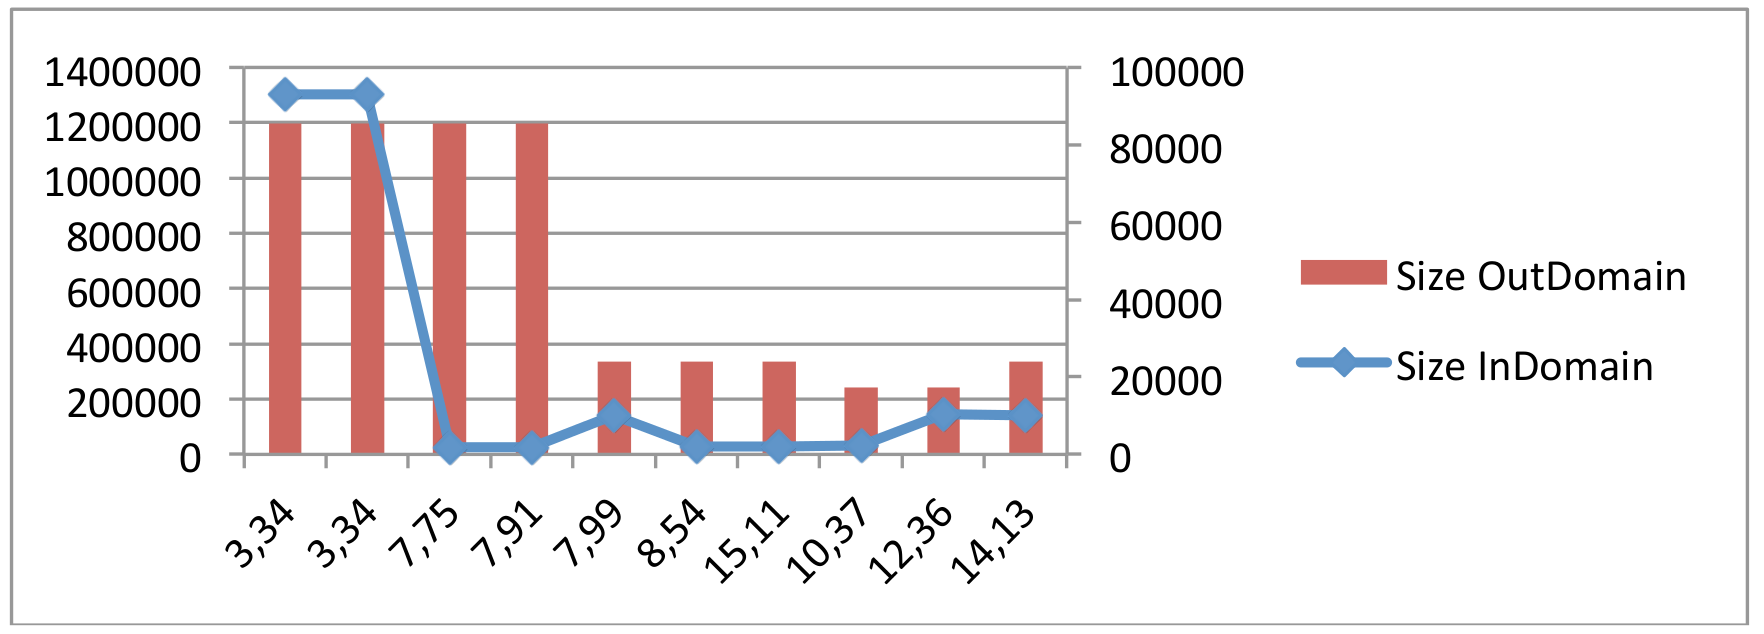
\includegraphics[width=\textwidth]{figures/DumaGraph1.png}
\label{fig:dumavertan:3}
\end{figure}


\largerpage
In \figref{fig:dumavertan:3} we plotted on the X axis the improvement, on the left Y axis the size of the out-of-domain data and on the second Y axis the size of the in-domain data.  
It can be observed that for the experiments that used large amounts of both out-of-domain and in-domain data, the improvement was the lowest. When the out-of-domain corpus and the in-domain corpus had smaller dimensions, the improvement was significantly better. Hybrid cases, with a large out-of-domain corpus and small in-domain corpus, can be observed in \figref{fig:dumavertan:4}, where all ten experiments are illustrated. In this case, the improvement is also significant. 

\begin{figure}
\caption{Improvement for all experiments}
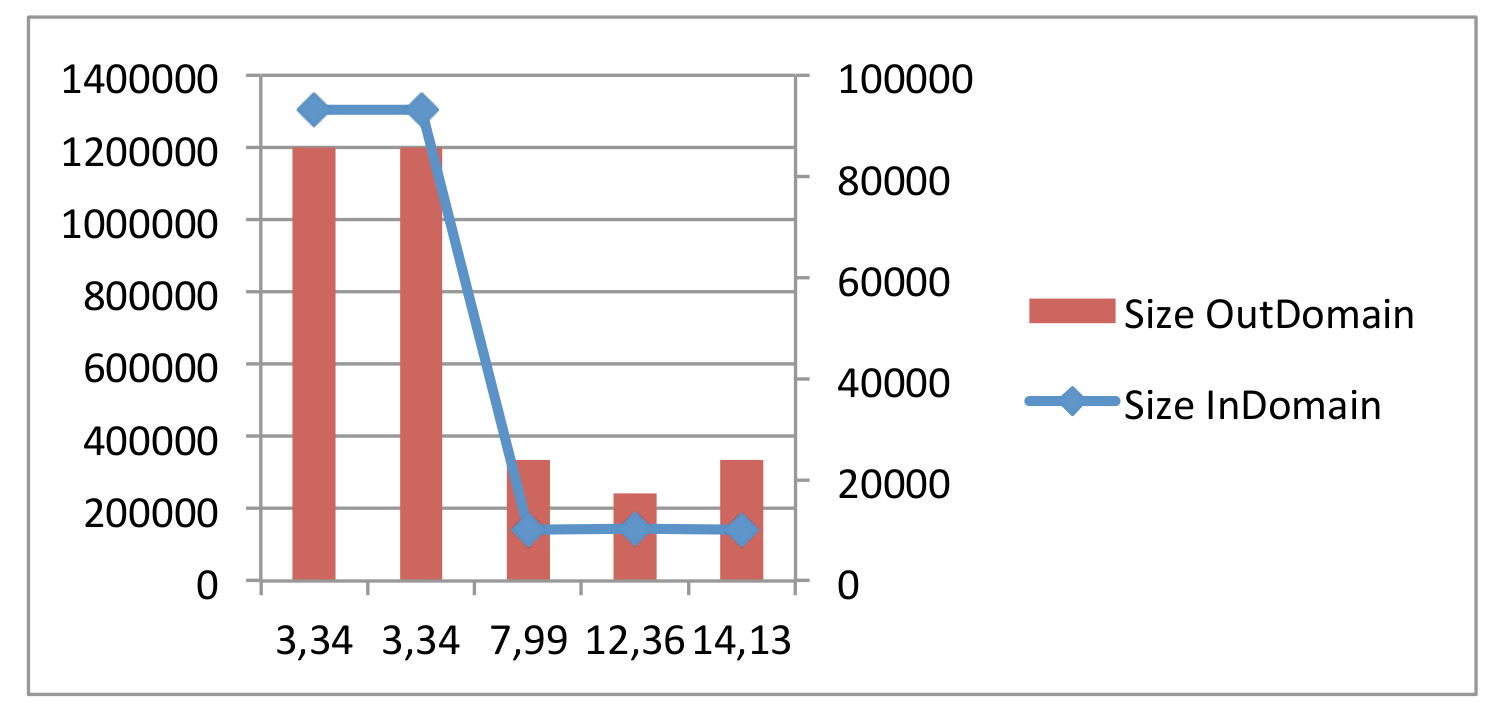
\includegraphics[width=\textwidth]{figures/DumaGraph2.png}
\label{fig:dumavertan:4}
\end{figure}

By looking at the improvements, we came to the conclusion that having more in-domain data does not necessarily lead to better results and that the chosen adaptation method is more important than the amount of in-domain data. 

In \tabref{tab:dumavertan:7}, an example of translations in the domain of Sociology and the language pair Romanian--English is presented. This is the experiment that gave the best improvement among all experiments (15.11). In the sentence translated using the baseline system, unknown words are underlined. The adapted system was able to translate all the words in this case and the sense of the sentence is similar to the sense of the reference sentence.

\begin{table}
 \begin{tabularx}{\textwidth}{lX}
\lsptoprule
{Type} &{Sentence}\\
\midrule
Source & toate declarațiile de susținere vor fi distruseîn termen de 18 luni de la  data de înregistrare a inițiativei propuse de cetățeni, sau, în cazul unor proceduri administrative sau juridice, cel târziu la o săptămână  după data încheierii procedurilor în cauză.\\
Reference & all statements of support will be destroyed at the latest 18 months after the date of registration of the proposed citizens' initiative, or, in the case of administrative or legal proceedings, at the latest one week after the date of conclusion of the said proceedings.\\
Adapted System & all statements of support will be destroyed 18 months after the registration of initiative proposed by citizens, or, in the case of administrative procedures or legal, at the latest one week after the date of the procedures in question.\\
Baseline System & all \underline{declarațiile} of \underline{susținere} shall be destroyed within 18 months from the date of registration of \underline{inițiativei} proposed by \underline{cetățeni}, or, in the case of administrative or legal, not later than one week from the date of conclusion of the procedures in question.\\
 \lspbottomrule
 \end{tabularx}
\caption{Translation example using a test set sentence that belongs to the Sociology domain, \textsc{ro--en}}
\label{tab:dumavertan:7}
\end{table}

\tabref{tab:dumavertan:8} presents an example taken from the Business domain German–English language pair test set. This is the experiment that gave the lowest improvement among all experiments (3.34). Even though in the sentence translated by the adapted system there are no unknown words, the sense of the sentence is not very close to the sense of the reference sentence.

\begin{table}
\begin{tabularx}{\textwidth}{lX}
\lsptoprule
{Type} &{Sentence}\\
\midrule
Source & eine solche anbindung birgt das risiko, dass aufwärtsgerichtete
inflationsschocks zu einer lohn-preis-spirale führen, was sich in
den betroffenen ländern nachteilig auf beschäftigung und
wettbewerbsfähigkeit auswirken würde.\\
Reference & such schemes involve the risk of upward shocks in inflation leading
to a wage-price spiral, which would be detrimental to employment
and competitiveness in the countries concerned.\\
Adapted System & such carries the risk that monetary policy discussion of an early,
in the countries concerned detrimental to employment and competitiveness.\\
Baseline System & such a link between carries the risk that \underline{aufwärtsgerichtete}
\underline{inflationsschocks} lead to a \underline{lohn-preis-spirale}, in the countries
concerned on employment and competitiveness.\\
\lspbottomrule
\end{tabularx}
\caption{Translation example using a test set sentence that belongs to the Business domain, \textsc{de--en}}
\label{tab:dumavertan:8}
\end{table}

\section{Conclusions}\label{section:6}

In this paper we presented the \textsc{atlas} Content Management System, focusing on the integration of machine translation into the system. A current problem of machine translation is domain adaptation, as many statistical systems are trained on a general domain and used on divergent domains. We have investigated three methods presented in \citet{Koehn2007} in order to choose a domain adaptation method that can be easily and quickly integrated into the system. According to the original article, the best adaption method  
among these three was the usage of an in-domain language model. However, our experiments show that in our current setting, the best method is language model interpolation.

Subsequently, we wanted to evaluate the chosen \textsc{da} method. For this reason, we performed experiments using baseline systems trained on \textsc{jrc}-Acquis and evaluated them using \textsc{bleu}.  In order to perform domain adaptation, we used the Business and Sociology in-domain data and the following language pairs: 
Ger\-man--English, 
English--German, 
Romanian--Bulgarian, 
English--Romanian, and 
Ro\-manian--English. The \textsc{bleu} scores for all the adapted systems outperformed the \textsc{bleu} scores of the baseline systems. It is important to emphasize the high \textsc{bleu} differences between the baseline systems and the adapted systems  (the best improvement was of 15.11 \textsc{bleu} points). 

Two important ideas are highlighted by the results of our experiments. When performing domain adaptation, it is not necessary to have a large in-domain corpus in order to attain good adaptation results (a size of 2000 sentences is sufficient). The other conclusion is that in our current setting, choosing the right method of adaptation is more important than having a large in-domain corpus.  

We conclude that having in-domain data is important for domain adaptation, but it is more important to choose a good adaptation method that gives significant improvements when applied to different in-domains and different language pairs. 

\section*{Acknowledgements}\label{sec:dumavertan:7}
 
\textsc{atlas} is a project funded by the European Commission under the \textsc{cip ict} Policy Support Program.

We want to thank the anonymous reviewers for their comments and constructive suggestions.

\sloppy
\printbibliography[heading=subbibliography,notkeyword=this]
\end{document}
